\documentclass[10pt]{beamer}
%% ── Thème sobre ──────────────────────────────────────────────────────
\usetheme{Madrid}
\usecolortheme{beaver}
\useinnertheme{rectangles}
\useoutertheme{infolines}

\definecolor{bleu}{RGB}{20,55,110}
\definecolor{bleulight}{RGB}{218,228,245}
\definecolor{bleumed}{RGB}{100,140,200}
\definecolor{gris}{RGB}{90,90,90}
\definecolor{rouge}{RGB}{160,30,30}
\definecolor{vert}{RGB}{50,200,50}

\setbeamercolor{structure}{fg=bleu}
\setbeamercolor{frametitle}{fg=bleu,bg=bleulight}
\setbeamercolor{title}{fg=white,bg=bleu}
\setbeamercolor{subtitle}{fg=bleulight}
\setbeamercolor{author in head/foot}{bg=bleu,fg=white}
\setbeamercolor{title in head/foot}{bg=bleu!80!black,fg=white}
\setbeamercolor{date in head/foot}{bg=bleu!60,fg=white}
\setbeamercolor{block title}{fg=white,bg=bleu}
\setbeamercolor{block body}{bg=bleulight!55}
\setbeamercolor{block title alerted}{fg=white,bg=bleu!75!black}
\setbeamercolor{block body alerted}{bg=bleulight!35}
\setbeamercolor{itemize item}{fg=bleu}
\setbeamercolor{itemize subitem}{fg=bleumed}
\setbeamercolor{enumerate item}{fg=bleu}

\setbeamerfont{frametitle}{series=\bfseries,size=\large,family=\rmfamily}
\setbeamerfont{title}{series=\bfseries,size=\Large,family=\rmfamily}
\setbeamerfont{block title}{series=\bfseries,family=\rmfamily}
\setbeamerfont{normal text}{family=\rmfamily}

\setbeamertemplate{navigation symbols}{}
\setbeamertemplate{itemize item}{$\bullet$}
\setbeamertemplate{itemize subitem}{$\circ$}

\setbeamertemplate{footline}{
	\leavevmode%
	\hbox{%
		\begin{beamercolorbox}[wd=.40\paperwidth,ht=2.25ex,dp=1ex,center]{author in head/foot}%
			\usebeamerfont{author in head/foot}\insertshortauthor
		\end{beamercolorbox}%
		\begin{beamercolorbox}[wd=.35\paperwidth,ht=2.25ex,dp=1ex,center]{title in head/foot}%
			\usebeamerfont{title in head/foot}\insertshorttitle
		\end{beamercolorbox}%
		\begin{beamercolorbox}[wd=.25\paperwidth,ht=2.25ex,dp=1ex,center]{date in head/foot}%
			\usebeamerfont{date in head/foot}\insertshortdate{}\hspace*{3em}
			\insertframenumber{} / \inserttotalframenumber\hspace*{2ex} 
	\end{beamercolorbox}}%
	\vbox{}%
}


%% ── Packages ─────────────────────────────────────────────────────────
\usepackage[utf8]{inputenc}
\usepackage[T1]{fontenc}

\usepackage{amsmath,amssymb,mathtools}
\usepackage{tikz}
\usetikzlibrary{arrows.meta,positioning,decorations.pathreplacing,calc,matrix,fit,backgrounds}
\usepackage{booktabs}
\usepackage{xcolor}
\usepackage{listings}
\usepackage{graphicx}

\lstset{
	language=Python,
	basicstyle=\ttfamily\scriptsize,
	keywordstyle=\color{bleu}\bfseries,
	commentstyle=\color{gris}\itshape,
	backgroundcolor=\color{bleulight!50},
	frame=single,framerule=0.4pt,rulecolor=\color{bleu!40},
	numbers=left,numberstyle=\tiny\color{gris},
	breaklines=true,showstringspaces=false
}

%% ── Macros ───────────────────────────────────────────────────────────
\newcommand{\ps}[2]{\langle #1,\, #2 \rangle}
\newcommand{\nm}[1]{\left\| #1 \right\|}
\newcommand{\RR}{\mathbb{R}}
\newcommand{\ZZ}{\mathbb{Z}}
\newcommand{\NN}{\mathbb{N}}
\renewcommand{\d}{\,\mathrm{d}}

%% ── Titre ────────────────────────────────────────────────────────────
\title{Transformée par ondelettes}
\subtitle{Et ses applications dans l'analyse d'images}
\author{De~Haese~Tao \and Piémontèse~Enzo \and Thirion~Louis}
\institute{Cité scolaire Carnot}
\date{TIPE 2026}

\begin{document}
	
	%%═══════════════════════════════════════════════════════════════════════
	%% DIAPO 1 — Titre
	%%═══════════════════════════════════════════════════════════════════════
	\begin{frame}
		\titlepage
	\end{frame}
	
	%%═══════════════════════════════════════════════════════════════════════
	%% DIAPO 2 — Plan (adapté aux nouvelles sections)
	%%═══════════════════════════════════════════════════════════════════════
	\begin{frame}{Plan et problématique}
		% [c] global pour que les milieux des deux colonnes soient alignés sur le milieu de la diapo
		\begin{columns}[c] 
			
			% Colonne de gauche (TDM)
			\begin{column}{0.55\textwidth}
				\tableofcontents
			\end{column}
			
			% Colonne de droite (Problématique)
			\begin{column}{0.45\textwidth}
				% \centering applique le centrage horizontal dans la colonne
				\centering 
				
				% On utilise une minipage pour réduire la largeur du bloc et 
				% créer un espace à gauche et à droite pour un centrage parfait
				\begin{minipage}{0.9\textwidth}
					\begin{alertblock}{Problématique}
						Comment compresser efficacement une image à l'aide des $\texttt{Ondelettes}$ analysantes ?
					\end{alertblock}
				\end{minipage}
				
			\end{column}
		\end{columns}
	\end{frame}
	
	%%═══════════════════════════════════════════════════════════════════════
	\section{Introduction à la compression d'images}
	%%═══════════════════════════════════════════════════════════════════════
	
	%%═══════════════════════════════════════════════════════════════════════
	%% DIAPO 3 — Qu'est-ce que compresser ?
	%%═══════════════════════════════════════════════════════════════════════
	\subsection{Qu'est ce que compresser une image ?}
	\begin{frame}{I — Qu'est-ce que compresser une image ?}
		
		\begin{columns}[T]
			\column{0.52\textwidth}
			Une image $N\!\times\!P$ en niveaux de gris : \\ $NP$ entiers dans $\{0,\ldots,255\}$.
			
			\medskip
			\textbf{Problème :} \\
			Stocker les coefficients \textit{importants} ; supprimer le reste tout en pouvant reconstruire.
			
			\medskip
			\textbf{Idée générale :} changer de représentation pour que
			\emph{peu de nombres} suffisent à décrire l'image.
			
			\medskip
			\begin{center}
				%% Remplacer par une photo : image_originale_vs_compressée.png
				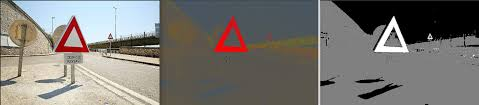
\includegraphics[scale=0.35]{Panneau.png}
			\end{center}
			
			\column{0.44\textwidth}
			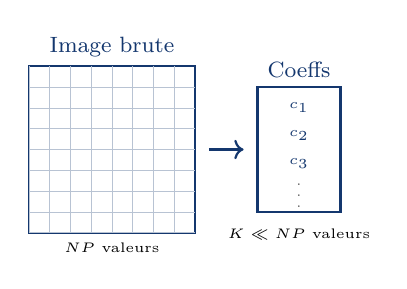
\begin{tikzpicture}[scale=0.88,font=\scriptsize]
				\draw[bleu,thick] (0,0) rectangle (2.4,2.4);
				\foreach \x in {0,0.3,...,2.3}
				\draw[bleu!30,very thin] (\x,0)--(\x,2.4);
				\foreach \y in {0,0.3,...,2.3}
				\draw[bleu!30,very thin] (0,\y)--(2.4,\y);
				\node[bleu,font=\footnotesize,above] at (1.2,2.4) {Image brute};
				\node[font=\tiny,below] at (1.2,0) {$NP$ valeurs};
				
				\draw[->,bleu,thick] (2.6,1.2)--(3.1,1.2);
				
				\begin{scope}[xshift=3.3cm,yshift=0.3cm]
					\draw[bleu,thick] (0,0) rectangle (1.2,1.8);
					\node[font=\tiny,text=bleu] at (0.6,1.5) {$c_1$};
					\node[font=\tiny,text=bleu] at (0.6,1.1) {$c_2$};
					\node[font=\tiny,text=bleu] at (0.6,0.7) {$c_3$};
					\node[font=\tiny,text=gris] at (0.6,0.35) {$\vdots$};
					\node[font=\tiny,below] at (0.6,-0.1) {$K \ll NP$ valeurs};
					\node[bleu,font=\footnotesize,above] at (0.6,1.8) {Coeffs};
				\end{scope}
			\end{tikzpicture}
			
			\medskip
			\begin{block}{Taux de compression}
				$\tau = \dfrac{\Omega}{NP}  < 1$ \\ $\Omega$ = coefficients nuls.
			\end{block}
			
		\end{columns}
	\end{frame}
	
	%%═══════════════════════════════════════════════════════════════════════
	%% DIAPO 4 — Deux stratégies sans transformée + limite
	%%═══════════════════════════════════════════════════════════════════════
	\subsection{Implémentation naïve}
	\begin{frame}{I — Deux stratégies sans transformée}
		
		\begin{columns}[T]
			\column{0.48\textwidth}
			\textbf{Codage entropique (Huffman)}\\[4pt]
			Les valeurs fréquentes reçoivent un code court.\\
			\underline{Exemple} :
			\begin{enumerate}
				\item Pixel gris foncé (fréquent) $\to$ \texttt{0}
				\item Pixel tout blanc (rare) $\to$ \texttt{110101}
			\end{enumerate}
			
			\medskip
			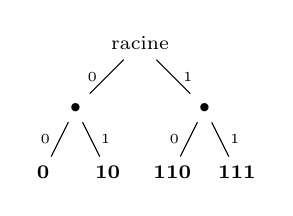
\begin{tikzpicture}[scale=0.82,font=\scriptsize,
				every node/.style={font=\scriptsize}]
				\node (r) at (2,3) {racine};
				\node (a) at (1,2) {$\bullet$};
				\node (b) at (3,2) {$\bullet$};
				\node (c) at (0.5,1) {\textbf{0}};
				\node (d) at (1.5,1) {\textbf{10}};
				\node (e) at (2.5,1) {\textbf{110}};
				\node (f) at (3.5,1) {\textbf{111}};
				\draw (r)--(a) node[midway,left]{\tiny 0};
				\draw (r)--(b) node[midway,right]{\tiny 1};
				\draw (a)--(c) node[midway,left]{\tiny 0};
				\draw (a)--(d) node[midway,right]{\tiny 1};
				\draw (b)--(e) node[midway,left]{\tiny 0};
				\draw (b)--(f) node[midway,right]{\tiny 1};
			\end{tikzpicture}
			
			\column{0.48\textwidth}
			\textbf{Codage prédictif (PNG, lossless)}\\[4pt]
			On prédit chaque pixel à partir de ses voisins et on code
			seulement l'\emph{erreur de prédiction}.
			
			\medskip
			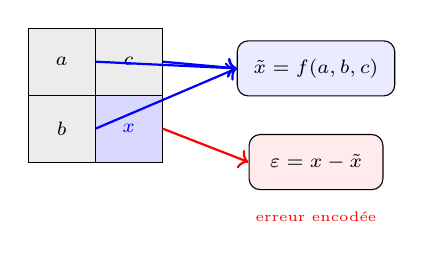
\begin{tikzpicture}[scale=0.85,font=\scriptsize,
				pixel/.style={draw,minimum size=0.85cm,align=center},
				known/.style={pixel,fill=gray!15},
				current/.style={pixel,fill=blue!15,text=blue}]
				\node[known]   (a) at (0,1) {$a$};
				\node[known]   (c) at (1,1) {$c$};
				\node[known]   (b) at (0,0) {$b$};
				\node[current] (x) at (1,0) {$x$};
				\node[draw,rounded corners,fill=blue!8,
				minimum width=2.0cm,minimum height=0.7cm] (pred) at (3.8,0.9)
				{$\tilde{x}=f(a,b,c)$};
				\node[draw,rounded corners,fill=red!8,
				minimum width=1.7cm,minimum height=0.7cm] (err) at (3.8,-0.5)
				{$\varepsilon = x-\tilde{x}$};
				\draw[->,thick,blue] (a.east)--(pred.west);
				\draw[->,thick,blue] (b.east)--(pred.west);
				\draw[->,thick,blue] (c.east)--(pred.west);
				\draw[->,thick,red]  (x.east)--(err.west);
				\node[red,font=\tiny,below] at (3.8,-1.1) {erreur encodée};
			\end{tikzpicture}
			
		\end{columns}
		
		\bigskip
		\begin{alertblock}{Limite commune — vers les transformées}
			Ces méthodes exploitent la \emph{redondance locale}, pas la structure globale.
			Une \textbf{transformation de l'image} concentre l'énergie en peu de coefficients
			et permet une compression bien plus efficace.
		\end{alertblock}
		
	\end{frame}
	
	%%═══════════════════════════════════════════════════════════════════════
	%% DIAPO 5 — Vers les ondelettes (remplace l'ancienne diapo DCT)
	%%═══════════════════════════════════════════════════════════════════════
	\subsection{Le changement de base}
	\begin{frame}{I — L'idée clé : changer de base}
		
		\textbf{Objectif :} trouver une représentation dans laquelle \emph{presque tous
			les coefficients sont nuls} — et ne garder que les importants.
		
		\begin{columns}[T]
			\column{0.52\textwidth}
			\begin{block}{Principe général}
				Soit $(e_k)$ une base orthonormée.  On projette :
				\[
				c_k = \ps{f}{e_k}
				\]
				On conserve les $K$ coefficients $c_k$ les plus grands et on met les autres à zéro.\\[4pt]
				\textbf{Clé :} choisir une base dans laquelle l'image transformée est \emph{creuse}.
			\end{block}
			
			\smallskip
			Une base idéale capte à la fois :\\
			$\bullet$ La \textbf{localisation spatiale} \\ 
			\textit{où est le détail ?}\\
			$\bullet$ La \textbf{fréquence} \\
			\textit{quelle échelle de variation ?}
			
			\column{0.44\textwidth}
			\begin{center}
				
				
				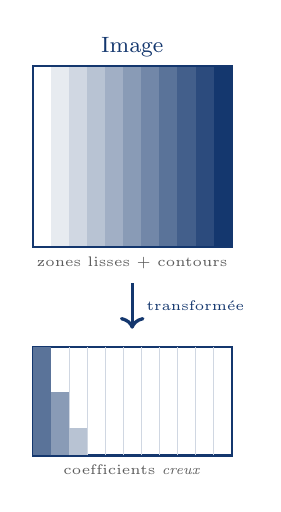
\begin{tikzpicture}[scale=1.15,font=\scriptsize]
					%% Image originale schématique
					\draw[bleu,thick,fill=bleulight!40] (0,2.3) rectangle (2.2,4.3);
					\node[bleu,font=\footnotesize,above] at (1.1,4.3) {Image};
					%% gradient horizontal simplifié
					\foreach \i in {0,1,...,10}{
						\fill[bleu!\the\numexpr10*\i\relax!white]
						({0.2*\i},2.3) rectangle ({0.2*\i+0.2},4.3);
					}
					\draw[bleu,thick] (0,2.3) rectangle (2.2,4.3);
					\node[gris,font=\tiny,below] at (1.1,2.3) {zones lisses + contours};
					
					%% flèche vers coefficients
					\draw[->,bleu,very thick] (1.1,1.9)--(1.1,1.4);
					\node[bleu,font=\tiny,right] at (1.15,1.65) {transformée};
					
					%% spectre creux
					\draw[bleu,thick] (0,0) rectangle (2.2,1.2);
					\foreach \x in {0.2,0.4,...,2.1}
					\draw[bleu!20,very thin] (\x,0)--(\x,1.2);
					%% quelques barres hautes
					\fill[bleu!70] (0.0,0) rectangle (0.2,1.2);
					\fill[bleu!50] (0.2,0) rectangle (0.4,0.7);
					\fill[bleu!30] (0.4,0) rectangle (0.6,0.3);
					%% reste quasi nul
					\node[gris,font=\tiny,below] at (1.1,0) {coefficients \emph{creux}};
				\end{tikzpicture}
			\end{center}
		\end{columns}
		
	\end{frame}
	
	%%═══════════════════════════════════════════════════════════════════════
	%% DIAPO 6 — Ligne directrice (remplace l'ancienne diapo JPEG→J2000)
	%%═══════════════════════════════════════════════════════════════════════
	\iffalse
	\begin{frame}{I — Ligne directrice}
		
		\begin{center}
			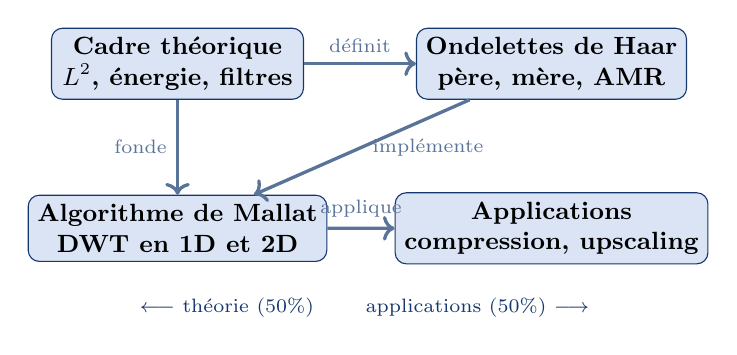
\begin{tikzpicture}[scale=0.95,font=\scriptsize,
				box/.style={draw=bleu,fill=bleulight,rounded corners,
					minimum width=3.2cm,minimum height=0.75cm,
					align=center,font=\small\bfseries},
				arr/.style={->,bleu!70,very thick}]
				
				\node[box] (A) at (0,0)    {Cadre théorique\\$L^2$, énergie, filtres};
				\node[box] (B) at (5,0)    {Ondelettes de Haar\\père, mère, AMR};
				\node[box] (C) at (0,-2.2) {Algorithme de Mallat\\DWT en 1D et 2D};
				\node[box] (D) at (5,-2.2) {Applications\\compression, upscaling};
				
				\draw[arr] (A)--(B) node[midway,above,font=\scriptsize]{définit};
				\draw[arr] (B)--(C) node[midway,right,font=\scriptsize]{implémente};
				\draw[arr] (A)--(C) node[midway,left,font=\scriptsize]{fonde};
				\draw[arr] (C)--(D) node[midway,above,font=\scriptsize]{applique};
				
				\node[bleu,font=\scriptsize,below] at (2.5,-3.0)
				{$\longleftarrow$ théorie (50\%) \quad\quad applications (50\%) $\longrightarrow$};
			\end{tikzpicture}
		\end{center}
		
		\medskip
		\begin{block}{Ce que nous allons montrer}
			$\bullet$ Pourquoi une \emph{base d'ondelettes} concentre l'énergie mieux qu'une
			base de Fourier pour les images naturelles.\\
			$\bullet$ Comment implémenter la transformée de Haar et s'en servir pour
			\textbf{compresser} et \textbf{agrandir} des images. \\
			$\bullet$ Les ondelettes fournissent une telle base : localisées en espace \emph{et}
			en fréquence, elles concentrent l'énergie des zones lisses en très peu de coefficients.
		\end{block}
		
	\end{frame}
	\fi
	%%═══════════════════════════════════════════════════════════════════════
	\section{II. Aspect théorique}
	%%═══════════════════════════════════════════════════════════════════════
	
	%%═══════════════════════════════════════════════════════════════════════
	%% DIAPO 7 — L^2, énergie, Parseval + illustration reconstruction
	%%═══════════════════════════════════════════════════════════════════════
	\subsection{Algèbre linéaire}
	\begin{frame}{II — Espace $L^2$, énergie et conservation}
		\vspace{-1.5em}
		\begin{columns}[T]
			\column{0.50\textwidth}
			\begin{block}{Algèbre linéaire}
				\[
				L^2(\RR) = \Bigl\{ f : \RR \to \RR \;\;;\;
				\int_\RR f^2 < +\infty \Bigr\}
				\]
				\[
				\ps{f}{g} = \int_\RR f(x)\,g(x)\d x
				\]
				\[
				\nm{f}^2 = \ps{f}{f} \triangleq \textit{Énergie}
				\]
				$\bullet$ C'est un espace préhilbertien complet. \\
				$\bullet$ \textbf{En dimension finie (discret) :} \\ on retrouve le \emph{PS} usuel de $\RR^N$ 
				
				\medskip
				
				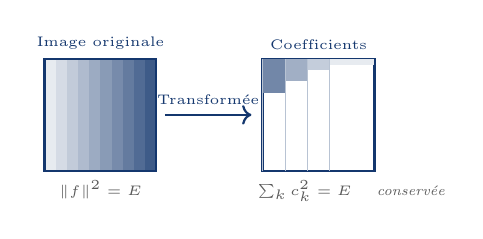
\begin{tikzpicture}[scale=0.71,font=\scriptsize]
					%% Image originale (gauche)
					\draw[bleu,thick,fill=bleulight!60] (0,1.5) rectangle (2,3.5);
					\node[bleu,font=\tiny,above] at (1,3.5) {Image originale};
					\foreach \i in {0,...,9}{
						\fill[bleu!\the\numexpr8*\i+10\relax!white]
						({0.2*\i},1.5) rectangle ({0.2*\i+0.2},3.5);
					}
					\draw[bleu,thick] (0,1.5) rectangle (2,3.5);
					\node[gris,font=\tiny,below] at (1,1.5) {$\nm{f}^2 = E$};
					
					%% flèche DWT
					\draw[->,bleu,thick] (2.15,2.5)--(3.7,2.5)
					node[midway,above,font=\tiny]{Transformée};
					
					%% Coefficients transformés (droite)
					\draw[bleu,thick] (3.9,1.5) rectangle (5.9,3.5);
					\fill[bleu!60] (3.9,2.9) rectangle (4.3,3.5);
					\fill[bleu!40] (4.3,3.1) rectangle (4.7,3.5);
					\fill[bleu!25] (4.7,3.3) rectangle (5.1,3.5);
					\fill[bleu!10] (5.1,3.4) rectangle (5.9,3.5);
					\foreach \x in {3.9,4.3,4.7,5.1}
					\draw[bleu!30,very thin] (\x,1.5)--(\x,3.5);
					\node[bleu,font=\tiny,above] at (4.9,3.5) {Coefficients};
					\node[gris,font=\tiny,below] at (5.5,1.5)
					{$\sum_k c_k^2 = E$ \quad\emph{conservée}};
				\end{tikzpicture}
				
			\end{block}
			
			
			\column{0.46\textwidth}
			
			
			\begin{alertblock}{Importance d'implémentation}
				La transformée doit être une \textbf{isométrie} $\Leftrightarrow$ conserve l'énergie. \\ Pour l'image cela se traduit par : \\
				Ne pas l’\textit{obscurcir} ou l’\textit{éclaircir} après transformation.
			\end{alertblock}
			
			\textbf{Illustration de l'isométrie}\\[4pt]
			
			\begin{center}
				%% Remplacer par une photo : image_originale_vs_compressée.png
				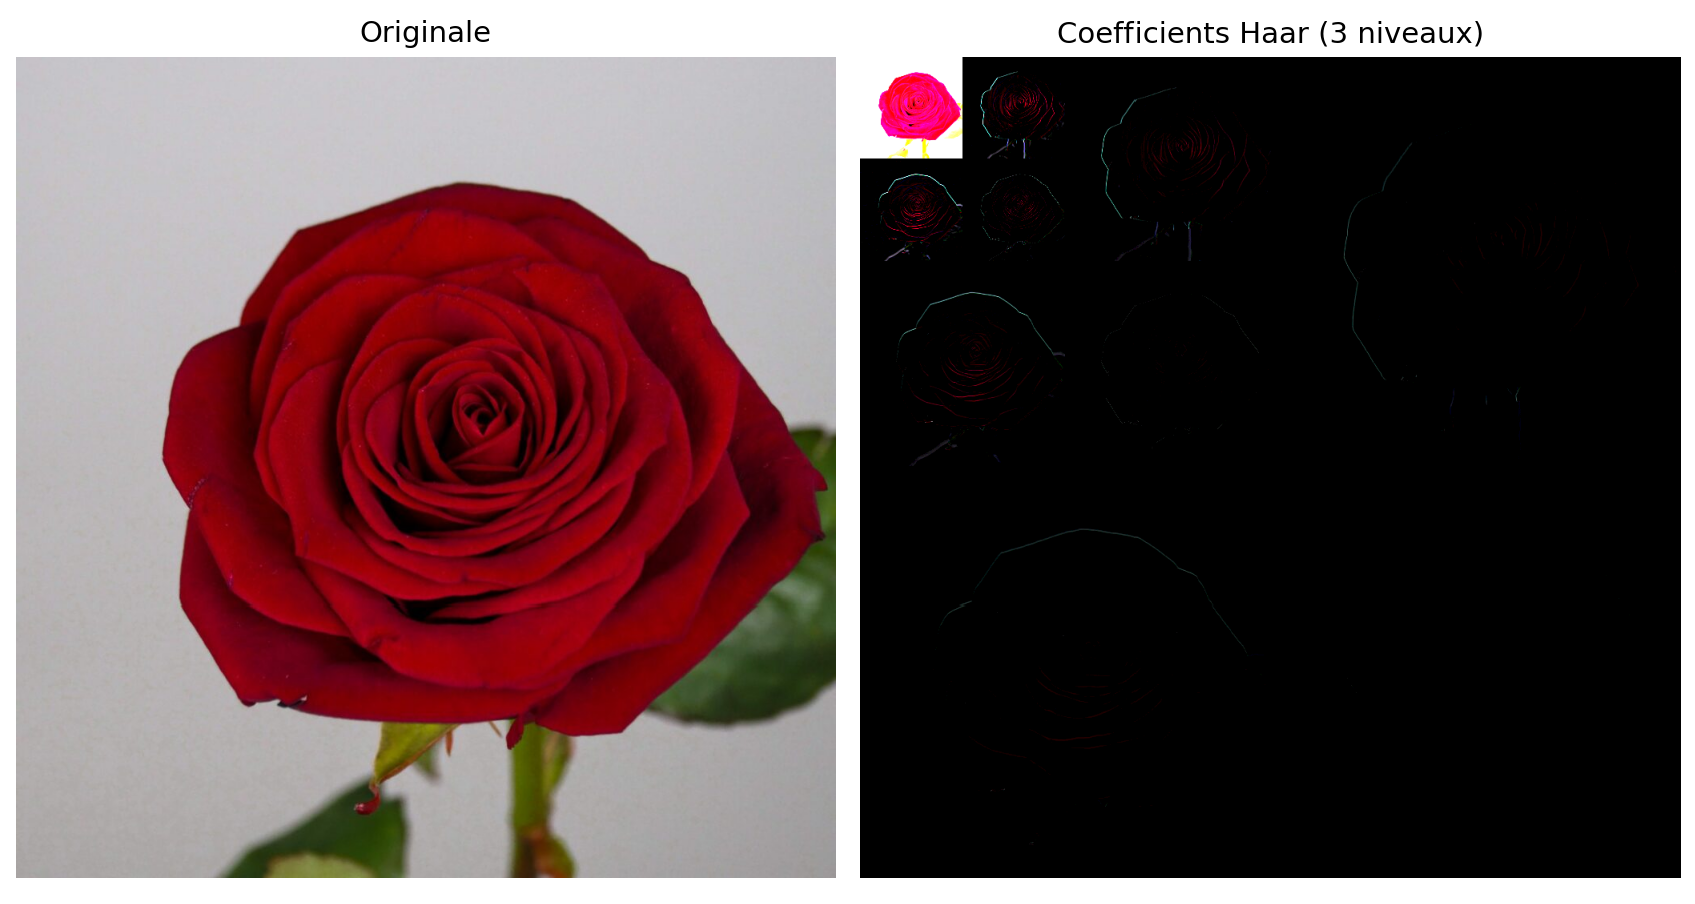
\includegraphics[scale=0.21]{compa.png}
			\end{center}
			
		\end{columns}
		
	\end{frame}
	
	%%═══════════════════════════════════════════════════════════════════════
	%% DIAPO 8 — Filtrage = produit scalaire
	%%═══════════════════════════════════════════════════════════════════════
	\begin{frame}[t]{II — Détecter les détails : filtrage et produit scalaire}
		
		\small Un signal peut être \textbf{décomposé} en :
		\begin{columns}[T]
			\column{0.50\textwidth}
			\begin{itemize}
				\item \small\textbf{tendances locales} \\$\Leftrightarrow$ \textbf{basses fréquences}
				\item \textbf{différences locales (détails)} \\$\Leftrightarrow$ \textbf{hautes fréquences}
			\end{itemize}
			Les ondelettes se comportent comme des \textbf{filtres} pour donner ces deux parties :
			\begin{itemize}
				\item \small\textbf{passe-bas} $\Rightarrow$ \textbf{tendances}
				\item \textbf{passe-haut} $\Rightarrow$ \textbf{détails}
			\end{itemize}
			\textbf{Exemple :}
			\begin{itemize}
				\item $h = \tfrac{1}{\sqrt{2}}(1,1)$ (passe-bas) :\\
				\item $g = \tfrac{1}{\sqrt{2}}(1,-1)$ (passe-haut) :\\
			\end{itemize}
			
			\column{0.46\textwidth}
			\begin{block}{En informatique}
				Les filtres sont représentés par des \textbf{vecteurs} et la réponse par le \textbf{produit scalaire usuel sur les matrices}.
			\end{block}
			
			\medskip
			
			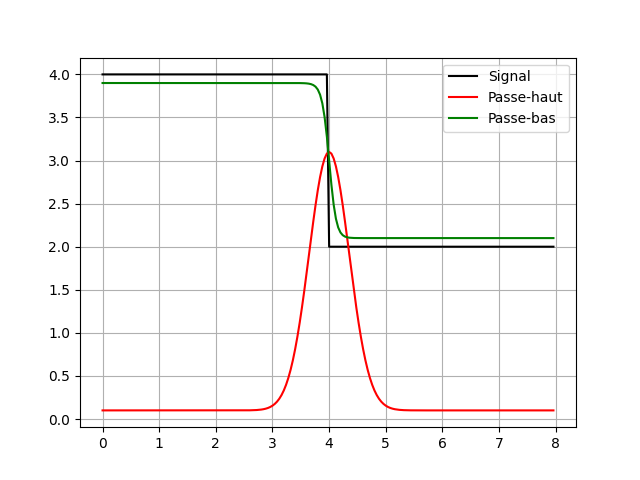
\includegraphics[scale=0.380]{filtres.png}
			
			
		\end{columns}
		
	\end{frame}
	
	%%═══════════════════════════════════════════════════════════════════════
	\subsection{Les ondelettes de Haar}
	%%═══════════════════════════════════════════════════════════════════════
	
	%%═══════════════════════════════════════════════════════════════════════
	%% DIAPO 9 — Père et mère de Haar
	%%═══════════════════════════════════════════════════════════════════════
	\begin{frame}{II — Fonctions de Haar : père et mère}
		\vspace{-0.6em}
		\begin{columns}[T]
			\column{0.46\textwidth}
			
			\begin{block}{Ondelette père $\varphi$ \scriptsize{(passe-bas)}}
				\[
				\varphi(x)=\begin{cases}1 & x\in[0,1[\\ 0& \text{sinon}\end{cases}
				\]
				\small Capture la \textbf{tendance} =
				\emph{moyenne locale}.
			\end{block}
			
			\begin{block}{Ondelette mère $\psi$ \scriptsize{(passe-haut)}}
				\[
				\psi(x)=\begin{cases}+1 & x\in[0,\tfrac{1}{2}[\\ -1 & x\in[\tfrac{1}{2},1[\\ 0 & \text{sinon}\end{cases}
				\]
				\small Capture les \textbf{détails} =
				\enph{différence locale}.
			\end{block}
			
			\begin{block}{Orthonormalité}
				\begin{enumerate}
					\item $\ps{\varphi}{\psi} = 0$ 
					\item $\nm{\varphi}=\nm{\psi}=1$
				\end{enumerate}
			\end{block}
			
			\column{0.50\textwidth}
			\begin{center}
				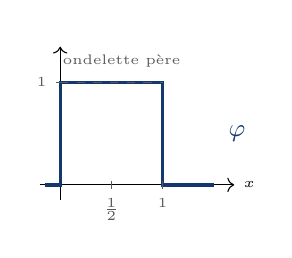
\begin{tikzpicture}[scale=1.3,font=\scriptsize]
					\draw[->](-0.2,0)--(1.7,0) node[right]{\tiny $x$};
					\draw[->](0,-0.15)--(0,1.35) node[above]{\tiny};
					\draw[bleu,very thick](-0.15,0)--(0,0)--(0,1)--(1,1)--(1,0)--(1.5,0);
					\draw[gris,dashed,thin](0,1)--(1,1);
					\draw[gris,thin](1,0.04)--(1,-0.04) node[below]{\tiny $1$};
					\draw[gris,thin](0.5,0.04)--(0.5,-0.04) node[below]{\tiny $\tfrac{1}{2}$};
					\draw[gris,thin](0.04,1)--(-0.04,1) node[left]{\tiny $1$};
					\node[bleu,right,font=\small] at (1.55,0.5){$\varphi$};
					\node[gris,font=\tiny,above] at (0.6,1.05){ondelette père};
				\end{tikzpicture}
			\end{center}
			\vspace{0.6em}
			
			\begin{center}
				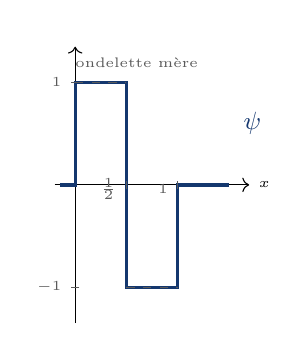
\begin{tikzpicture}[scale=1.3,font=\scriptsize]
					\draw[->](-0.2,0)--(1.7,0) node[right]{\tiny $x$};
					\draw[->](0,-1.35)--(0,1.35) node[above]{\tiny};
					\draw[bleu,very thick]
					(-0.15,0)--(0,0)--(0,1)--(0.5,1)--(0.5,-1)--(1,-1)--(1,0)--(1.5,0);
					\draw[gris,dashed,thin](0,1)--(0.5,1);
					\draw[gris,dashed,thin](0.5,-1)--(1,-1);
					\draw[gris,thin](1,0.04)--(1,-0.04) node[left]{\tiny $1$};
					\draw[gris,thin](0.5,0.04)--(0.5,-0.04) node[left]{\tiny $\tfrac{1}{2}$};
					\draw[gris,thin](0.04,1)--(-0.04,1) node[left]{\tiny $1$};
					\draw[gris,thin](0.04,-1)--(-0.04,-1) node[left]{\tiny $-1$};
					\node[bleu,right,font=\small] at (1.55,0.6){$\psi$};
					\node[gris,font=\tiny,above] at (0.6,1.05){ondelette mère};
				\end{tikzpicture}
			\end{center}
		\end{columns}
		
	\end{frame}
	
	%%═══════════════════════════════════════════════════════════════════════
	%% DIAPO 10 — Fils et filles : translations et dilatations
	%%═══════════════════════════════════════════════════════════════════════
	\begin{frame}{II — Fils et filles : translations et dilatations}
		
		À partir de $\varphi$ et $\psi$, on génère une famille indexée par
		l'\textbf{échelle} $j$ et la \textbf{position} $k$ :
		\[
		\varphi_{j,k}(x)=2^{j/2}\varphi \left( 2^j \big( x-\frac{k}{2^j} \big) \right), \quad
		\psi_{j,k}(x)=2^{j/2}\psi \left( 2^j \big( x-\frac{k}{2^j} \big) \right) , \quad (k,j) \in \ZZ \times \NN
		\]
		
		\begin{columns}[T]
			\column{0.43\textwidth}
			\begin{itemize}
				\item $j$ grand $\Rightarrow$ fenêtre \emph{fine} (HF)
				\item $k$ décale la position de $k\cdot 2^{-j}$
				\item $2^{j/2}$ normalise : $\nm{\psi_{j,k}}=1$
			\end{itemize}
			
			\medskip
			\begin{block}{Base complète}
				$\{\varphi_{0,k}\}_{k\in\ZZ}\cup\{\psi_{j,k}\}_{j\geq0,k\in\ZZ}$
				est une base orthonormée de $L^2(\RR)$.
				\[
				f = \sum_k c_k\,\varphi_{0,k} + \sum_{j\geq0}\sum_k d_{j,k}\,\psi_{j,k}
				\]
			\end{block}
			
			\column{0.53\textwidth}
			\begin{center}
				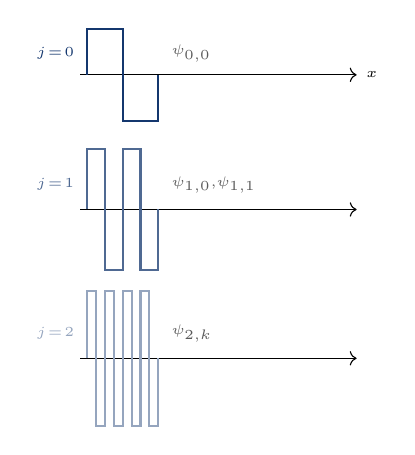
\begin{tikzpicture}[scale=0.9,font=\scriptsize]
					\draw[->](-0.1,0)--(3.8,0) node[right]{\tiny $x$};
					\draw[bleu,thick]
					(0,0)--(0,0.65)--(0.5,0.65)--(0.5,-0.65)--(1,-0.65)--(1,0);
					\node[bleu,left,font=\tiny] at (-0.05,0.3){$j\!=\!0$};
					\node[gris,font=\tiny,right] at (1.05,0.3){$\psi_{0,0}$};
					
					\begin{scope}[yshift=-1.9cm]
						\draw[->](-0.1,0)--(3.8,0);
						\draw[bleu!75,thick]
						(0,0)--(0,0.85)--(0.25,0.85)--(0.25,-0.85)--(0.5,-0.85)--(0.5,0);
						\draw[bleu!75,thick]
						(0.5,0)--(0.5,0.85)--(0.75,0.85)--(0.75,-0.85)--(1,-0.85)--(1,0);
						\node[bleu!75,left,font=\tiny] at (-0.05,0.35){$j\!=\!1$};
						\node[gris,font=\tiny,right] at (1.05,0.35){$\psi_{1,0}$,$\psi_{1,1}$};
					\end{scope}
					
					\begin{scope}[yshift=-4.0cm]
						\draw[->](-0.1,0)--(3.8,0);
						\foreach \kk in {0,1,2,3}{
							\draw[bleu!45,thick]
							({0.25*\kk},0)--({0.25*\kk},0.95)
							--({0.25*\kk+0.125},0.95)
							--({0.25*\kk+0.125},-0.95)
							--({0.25*\kk+0.25},-0.95)
							--({0.25*\kk+0.25},0);
						}
						\node[bleu!45,left,font=\tiny] at (-0.05,0.35){$j\!=\!2$};
						\node[gris,font=\tiny,right] at (1.05,0.35){$\psi_{2,k}$};
					\end{scope}
				\end{tikzpicture}
			\end{center}
		\end{columns}
		
	\end{frame}
	
	%%═══════════════════════════════════════════════════════════════════════
	%% DIAPO 11 — Propriétés d'orthogonalité + AMR
	%%═══════════════════════════════════════════════════════════════════════
	\subsection{Analyse multi-résolution}
	\begin{frame}{II — Propriétés et analyse multi-résolution (AMR)}
		
		\begin{columns}[T]
			\column{0.52\textwidth}
			
			\begin{block}{Orthogonalité}
				$ \forall (j,j',k,k') \in \NN^2 \times \ZZ ^2$ :
				\[
				\ps{\varphi_{j,k}}{\varphi_{j,k'}} =
				\ps{\psi_{j,k}}{\psi_{j,k'}} = \delta_{kk'}
				\]
				\[
				\ps{\varphi_{j,k}}{\psi_{j',k'}} = 0 
				\]
			\end{block}
			
			\medskip
			\begin{block}{Espaces emboîtés}
				On pose V_j = \mathrm{Vect}\{\varphi_{j,k}\}_{k\in [|0,2^j-1|]}\\
				\qquad \quad \; W_j = \mathrm{Vect}\{\psi_{j,k}\}_{k\in [|0,2^j-1|]}
				\vspace{0.6em}
				$
				\cdots\subset V_0\subset V_1\subset V_2\subset\cdots\subset L^2(\RR) 
				$
				\[
				V_{j+1} = V_j \overset{\perp}{\oplus} W_j
				\]
				En itérant : $\;V_J = V_0\oplus W_0\oplus\cdots\oplus W_{J-1}$
			\end{block}
			
			
			\column{0.44\textwidth}
			
			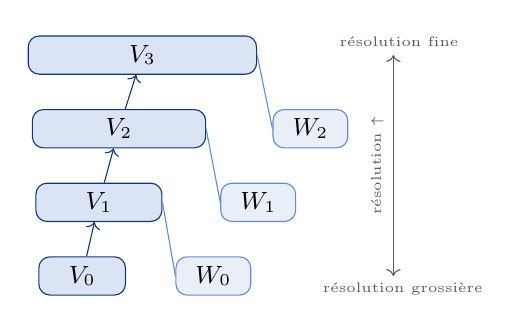
\begin{tikzpicture}[scale=0.85,font=\small]
				\node[draw=bleu,fill=bleulight,rounded corners,
				minimum width=2.9cm,minimum height=0.45cm,align=center]
				(V3) at (1.45,4.0){$V_3$};
				\node[draw=bleu,fill=bleulight,rounded corners,
				minimum width=2.2cm,minimum height=0.45cm,align=center]
				(V2) at (1.1,2.9){$V_2$};
				\node[draw=bleumed,fill=bleulight!60,rounded corners,
				minimum width=0.95cm,minimum height=0.45cm,align=center]
				(W2) at (3.96,2.9){$W_2$};
				\node[draw=bleu,fill=bleulight,rounded corners,
				minimum width=1.6cm,minimum height=0.45cm,align=center]
				(V1) at (0.8,1.8){$V_1$};
				\node[draw=bleumed,fill=bleulight!60,rounded corners,
				minimum width=0.95cm,minimum height=0.45cm,align=center]
				(W1) at (3.18,1.8){$W_1$};
				\node[draw=bleu,fill=bleulight,rounded corners,
				minimum width=1.1cm,minimum height=0.45cm,align=center]
				(V0) at (0.55,0.7){$V_0$};
				\node[draw=bleumed,fill=bleulight!60,rounded corners,
				minimum width=0.95cm,minimum height=0.45cm,align=center]
				(W0) at (2.51,0.7){$W_0$};
				\draw[->,bleu](V2)--(V3);
				\draw[->,bleu](V1)--(V2);
				\draw[->,bleu](V0)--(V1);
				\draw[bleumed](W2.west)--(V3.east);
				\draw[bleumed](W1.west)--(V2.east);
				\draw[bleumed](W0.west)--(V1.east);
				\node[gris,font=\tiny,right] at (4.25,4.2){résolution fine};
				\node[gris,font=\tiny,right] at (4,0.5){résolution grossière};
				\draw[<->,gris,thin](5.2,0.7)--(5.2,4.0)
				node[midway,right,font=\tiny,rotate=90,anchor=south]{résolution $\uparrow$};
			\end{tikzpicture}
			
			\medskip
			\begin{block}{Interprétation}
				$V_j$ = image \emph{lissée} à l'échelle $2^{-j}$\par
				$W_j$ = détails à l'échelle $2^{-j}$\\
				
				\fcolorbox{red}{bleulight!55}{%
					\parbox{0.8\textwidth}{Seuiller $W_j$ $\Leftrightarrow$ supprimer les petits détails}}
				
			\end{block}
			
		\end{columns}
		
	\end{frame}
	
	%%═══════════════════════════════════════════════════════════════════════
	
	%%═══════════════════════════════════════════════════════════════════════
	%% DIAPO 12 — Exemple 1D Haar
	%%═══════════════════════════════════════════════════════════════════════
	\begin{frame}{II — Exemple 1D : décomposition de Haar}
		
		\textbf{Signal $N=8$ :} $\;[2\ \ 4\ \ 8\ \ 12\ \ 14\ \ 0\ \ 2\ \ 1]$
		
		\begin{center}
			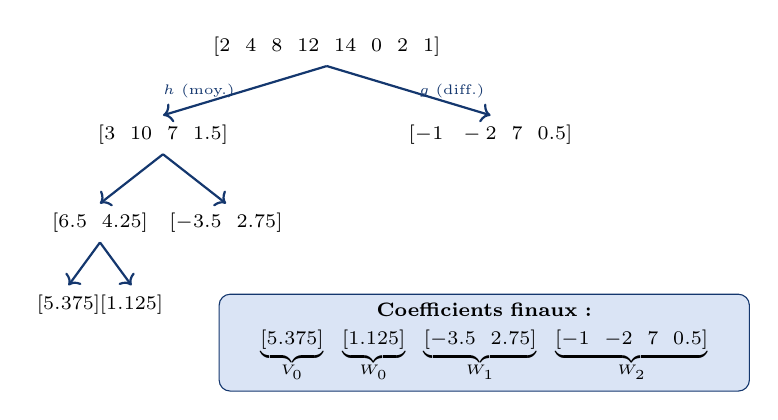
\begin{tikzpicture}[scale=0.80,font=\scriptsize,
				arr/.style={->,bleu,thick}]
				\node (s0) at (0,3.8){$[2\ \ 4\ \ 8\ \ 12\ \ 14\ \ 0\ \ 2\ \ 1]$};
				
				\node (a1) at (-2.6,2.4){$[3\ \ 10\ \ 7\ \ 1.5]$};
				\node (d1) at (2.6,2.4){$[-1\ \ -2\ \ 7\ \ 0.5]$};
				\draw[arr](s0.south)--(a1.north) node[midway,left,font=\tiny]{$h$ (moy.)};
				\draw[arr](s0.south)--(d1.north) node[midway,right,font=\tiny]{$g$ (diff.)};
				
				\node (a2) at (-3.6,1.0){$[6.5\ \ 4.25]$};
				\node (d2) at (-1.6,1.0){$[-3.5\ \ 2.75]$};
				\draw[arr](a1.south)--(a2.north);
				\draw[arr](a1.south)--(d2.north);
				
				\node (a3) at (-4.1,-0.3){$[5.375]$};
				\node (d3) at (-3.1,-0.3){$[1.125]$};
				\draw[arr](a2.south)--(a3.north);
				\draw[arr](a2.south)--(d3.north);
				
				\node[draw=bleu,fill=bleulight,rounded corners,align=center,
				font=\scriptsize,text width=6.5cm] at (2.5,-0.9){
					\textbf{Coefficients finaux :}\\[2pt]
					$\underbrace{[5.375]}_{V_0}\ \
					\underbrace{[1.125]}_{W_0}\ \
					\underbrace{[-3.5\ \ 2.75]}_{W_1}\ \
					\underbrace{[-1\ \ {-2}\ \ 7\ \ 0.5]}_{W_2}$
				};
			\end{tikzpicture}
		\end{center}
		\medskip
		\begin{alertblock}{Conclusion sur Haar}
			\small $\bullet$ Les détails ($W_j$) tendent vers zéro sur les zones lisses $\to$ idéal pour la compression. \\
			$\bullet$ On peut coder la transformée en \textbf{Python} et son inverse
		\end{alertblock}
		
	\end{frame}
	
	%%═══════════════════════════════════════════════════════════════════════
	%% DIAPO 13 — Généralisation 2D
	%%═══════════════════════════════════════════════════════════════════════
	\begin{frame}{II — Généralisation 2D : les quatre sous-bandes}
		
		\textbf{Principe :} filtrer les \emph{lignes} puis les \emph{colonnes}. On peut répéter l'opération sur plusieurs niveaux en repartant de la sous-bande d'approximation. 
		
		\begin{columns}[T]
			\column{0.50\textwidth}
			
			\begin{center}
				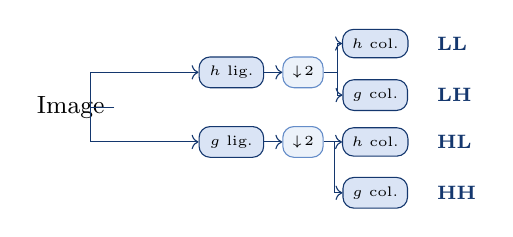
\begin{tikzpicture}[scale=0.85,font=\scriptsize]
					\node[font=\small, left] (im) at (0,0){Image};
					\node[draw=bleu,fill=bleulight,rounded corners,font=\tiny,
					minimum width=0.82cm,minimum height=0.36cm](hl) at (1.75,0.52){$h$ lig.};
					\node[draw=bleu,fill=bleulight,rounded corners,font=\tiny,
					minimum width=0.82cm,minimum height=0.36cm](gl) at (1.75,-0.52){$g$ lig.};
					\node[draw=bleumed,fill=bleulight!50,rounded corners,font=\tiny,
					minimum width=0.48cm,minimum height=0.36cm](d2h) at (2.82,0.52){$\downarrow\!2$};
					\node[draw=bleumed,fill=bleulight!50,rounded corners,font=\tiny,
					minimum width=0.48cm,minimum height=0.36cm](d2g) at (2.82,-0.52){$\downarrow\!2$};
					\node[draw=bleu,fill=bleulight,rounded corners,font=\tiny,
					minimum width=0.82cm,minimum height=0.36cm](hc1) at (3.9,0.95){$h$ col.};
					\node[draw=bleu,fill=bleulight,rounded corners,font=\tiny,
					minimum width=0.82cm,minimum height=0.36cm](gc1) at (3.9,0.18){$g$ col.};
					\node[draw=bleu,fill=bleulight,rounded corners,font=\tiny,
					minimum width=0.82cm,minimum height=0.36cm](hc2) at (3.9,-0.52){$h$ col.};
					\node[draw=bleu,fill=bleulight,rounded corners,font=\tiny,
					minimum width=0.82cm,minimum height=0.36cm](gc2) at (3.9,-1.28){$g$ col.};
					\node[font=\scriptsize,bleu,right] at (4.68,0.95){\textbf{LL}};
					\node[font=\scriptsize,bleu,right] at (4.68,0.18){\textbf{LH}};
					\node[font=\scriptsize,bleu,right] at (4.68,-0.52){\textbf{HL}};
					\node[font=\scriptsize,bleu,right] at (4.68,-1.28){\textbf{HH}};
					\draw[->,bleu](im)--++(0.3,0) |- (hl);
					\draw[->,bleu](im)--++(0.3,0) |- (gl);
					\draw[->,bleu](hl)--(d2h); \draw[->,bleu](gl)--(d2g);
					\draw[->,bleu](d2h.east)--++(0.2,0) |- (hc1);
					\draw[->,bleu](d2h.east)--++(0.2,0) |- (gc1);
					\draw[->,bleu](d2g.east)--++(0.16,0) |- (hc2);
					\draw[->,bleu](d2g.east)--++(0.16,0) |- (gc2);
				\end{tikzpicture}
			\end{center}
			
			\vspace{0.2em}
			\begin{tabular}{@{}ll@{}}
				\toprule
				Sous-bande & Contenu \\
				\midrule
				\textbf{LL} & Approximation (BF) \\
				\textbf{LH} & Contours horizontaux \\
				\textbf{HL} & Contours verticaux \\
				\textbf{HH} & Détails diagonaux \\
				\bottomrule
			\end{tabular}
			
			\column{0.46\textwidth}
			\begin{center}
				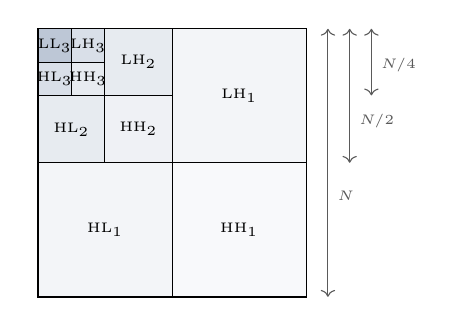
\begin{tikzpicture}[scale=0.92,font=\scriptsize]
					\draw[fill=white,draw=black,thick](0,0) rectangle (3.7,3.7);
					
					\draw[fill=bleu!28](0,3.24) rectangle (0.46,3.7) node[midway,font=\tiny]{LL$_3$};
					\draw[fill=bleu!16](0.46,3.24) rectangle (0.92,3.7) node[midway,font=\tiny]{LH$_3$};
					\draw[fill=bleu!16](0,2.78) rectangle (0.46,3.24) node[midway,font=\tiny]{HL$_3$};
					\draw[fill=bleu!10](0.46,2.78) rectangle (0.92,3.24) node[midway,font=\tiny]{HH$_3$};
					
					\draw[fill=bleu!10](0.92,2.78) rectangle (1.85,3.7) node[midway,font=\tiny]{LH$_2$};
					\draw[fill=bleu!10](0,1.84) rectangle (0.92,2.78) node[midway,font=\tiny]{HL$_2$};
					\draw[fill=bleu!07](0.92,1.85) rectangle (1.85,2.78) node[midway,font=\tiny]{HH$_2$};
					
					\draw[fill=bleu!05](1.85,1.85) rectangle (3.7,3.7) node[midway,font=\tiny]{LH$_1$};
					\draw[fill=bleu!05](0,0) rectangle (1.85,1.85) node[midway,font=\tiny]{HL$_1$};
					\draw[fill=bleu!03](1.85,0) rectangle (3.7,1.85) node[midway,font=\tiny]{HH$_1$};
					
					\draw[<->,gris,thin](4,3.7)--(4,0) node[midway,right,yshift=-12pt,font=\tiny]{$N$};
					\draw[<->,gris,thin](4.3,3.7)--(4.3,1.85) node[midway,right,yshift=-9pt,font=\tiny]{$N/2$};
					\draw[<->,gris,thin](4.6,3.7)--(4.6,2.78) node[midway,right,yshift=-1pt,font=\tiny]{$N/4$};
				\end{tikzpicture}
			\end{center}
			
			\vspace*{-10pt}
			\begin{block}{Conséquences}
				\small $\bullet$ L'énergie se concentre dans les sous-bandes \textbf{LL}. On peut seuiller intelligemment sans trop de \textit{dégâts} \\ 
				$\bullet$ L'implémentation \textbf{Python} 2D se réalise à partir de celle en 1D. 
			\end{block}
			
		\end{columns}
		
	\end{frame}
	
	%%═══════════════════════════════════════════════════════════════════════
	\section{III. Pratique }
	%%═══════════════════════════════════════════════════════════════════════
	\subsection{Images en couleurs}
	\begin{frame}[t]{III -- Images en couleurs}
		
		\begin{columns}[T]
			
			\column{0.45\textwidth}
			\centering
			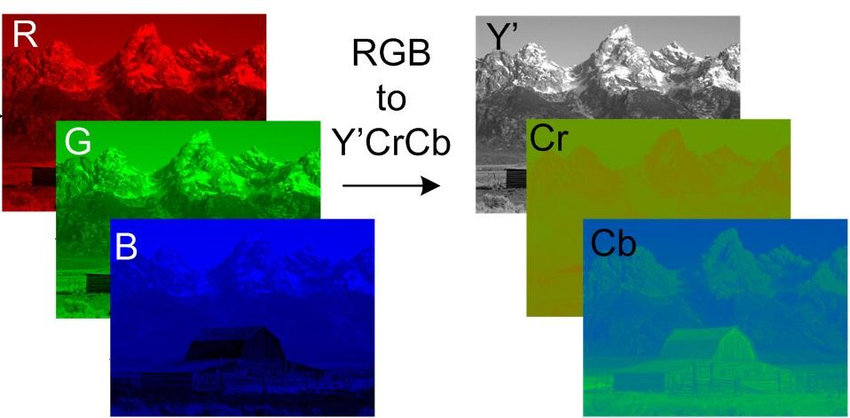
\includegraphics[width=\linewidth]{RGB-YCC.png}
			
			\vspace{-0.4cm}
			
			\column{0.55\textwidth}
			
			\textbf{Espace RGB :}
			\begin{itemize}
				\item Trois canaux : Rouge, Vert, Bleu.
			\end{itemize}
			
			\smallskip
			
			\textbf{Espace YCbCr :}
			\begin{itemize}
				\item $Y$ : luminance (niveau de gris).
				\item $Cb$ et $Cr$ : canaux chromatiques
				\item \small Œil humain + sensible à $Y$ que $Cb$ / $Cr$.
			\end{itemize}
			
		\end{columns}
		
		\vspace{0.4cm}
		
		\centering
		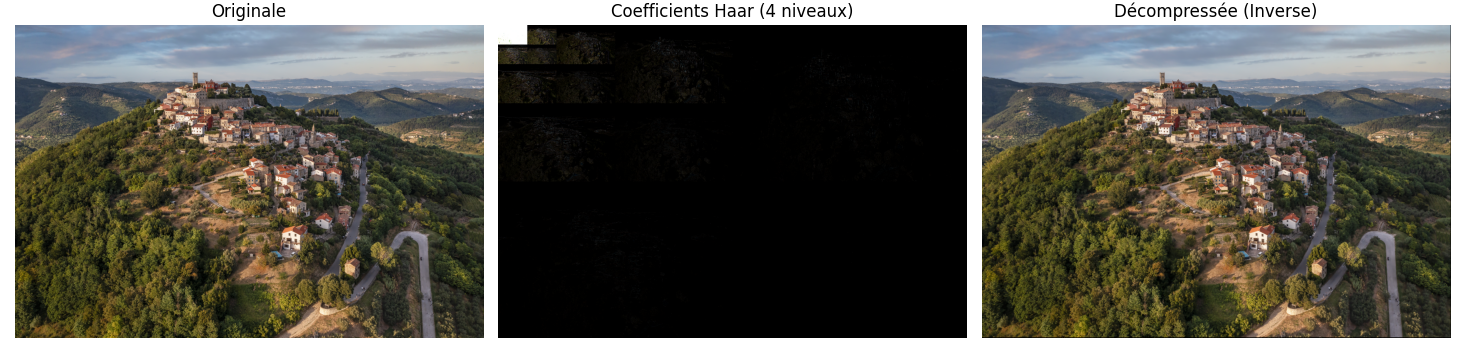
\includegraphics[width=\linewidth]{village_couleurs.png}
		
		\begin{center}
			La généralisation aux couleurs passe par la transformation de chacun des canaux.
		\end{center}
		
	\end{frame}
	%%═══════════════════════════════════════════════════════════════════════
	%% DIAPO 14 — Seuillage et lien avec l'énergie
	%%═══════════════════════════════════════════════════════════════════════
	\subsection{Compression}
	\subsubsection{Seuillage}
	\begin{frame}{III — Compression : seuillage et énergie}
		
		\textbf{Après la DWT, compresser = annuler les petits coefficients.}
		
		\begin{columns}[T]
			\column{0.50\textwidth}
			
			\underline{Seuillage dur :}  {\scriptsize  (Introduit une \emph{discontinuité})}
			\[
			\bar{c} = \begin{cases} c & |c|\geq\lambda \\ 0 & |c|<\lambda \end{cases} 
			\]
			\underline{Seuillage doux :}  {\scriptsize  (Introduit une \emph{perte d'énergie})}
			\[ \bar{c} = \mathrm{sgn}(c)\max(|c|-\lambda,0) 
			\]
			
			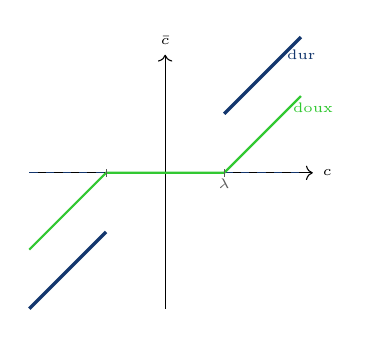
\begin{tikzpicture}[scale=0.75]
				\draw[->](-2.3,0)--(2.5,0) node[right]{\tiny $c$};
				\draw[->](0,-2.3)--(0,2.0) node[above]{\tiny $\bar c$};
				\draw[bleu,very thick](-2.3,-2.3)--(-1,-1);
				\draw[bleu,very thick](1,1)--(2.3,2.3);
				\draw[bleu,dashed](-2.3,0)--(-1,0) (1,0)--(2.3,0);
				\draw[vert,thick](-2.3,-1.3)--(-1,0)--(1,0)--(2.3,1.3);
				\draw[gris,thin](1,-0.07)--(1,0.07) node[below,font=\tiny]{$\lambda$};
				\draw[gris,thin](-1,-0.07)--(-1,0.07);
				\node[bleu,font=\tiny,right] at (1.9,2.0){dur};
				\node[vert,font=\tiny,right] at (2,1.1){doux};
			\end{tikzpicture}
			
			\column{0.46\textwidth}
			\begin{block}{Erreur contrôlée}
				\[
				\nm{f-\bar{f}}^2 = \sum_{\bar{c}_k=0} c_k^2
				\]
				\begin{enumerate}
					\item On choisit $\lambda$ pour contrôler \emph{l'erreur quadratique totale.}
					\item Il existe des ondelettes (Cohen–Daubechies–Feauveau), où l'on peut seuiller  plus fort.
					\item On ne seuille pas la sous-bande LL$_n$ (\emph{énergie principale}).
				\end{enumerate}
			\end{block}
			
			
			\textit{Notre implémentation utilise le \textbf{seuillage dur}.}
			
		\end{columns}
		
	\end{frame}
	
	\begin{frame}{III —  Résultats expérimentaux : Effet du seuillage}
		
		\begin{columns}[T]
			
			\column{0.33\textwidth}
			\centering
			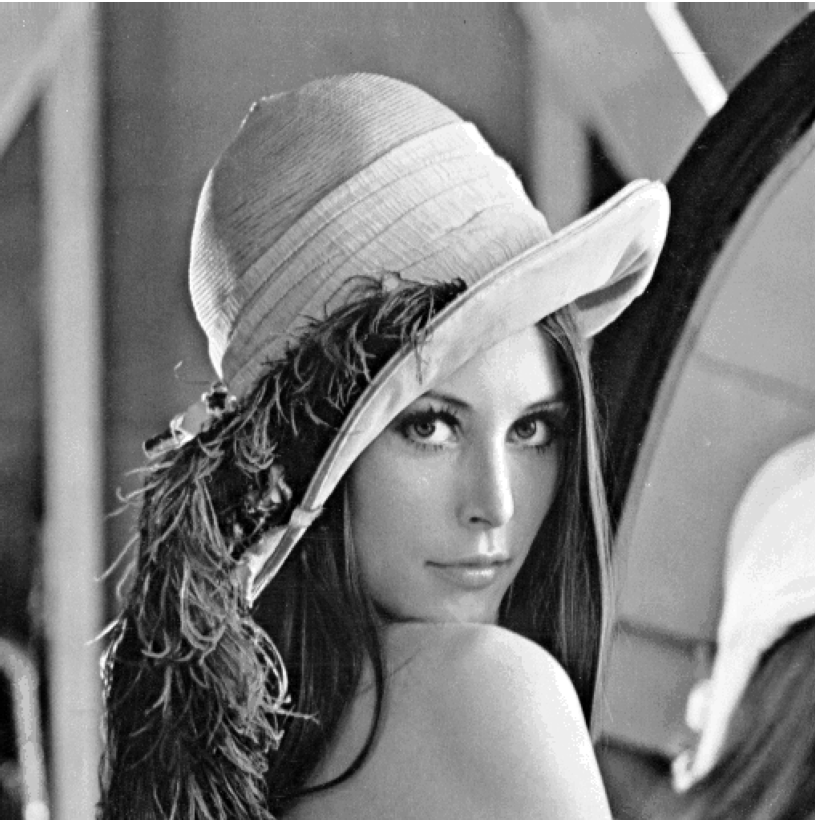
\includegraphics[width=\linewidth]{Lena_0.png}
			
			\vspace{0.2cm}
			{\color{bleu}\bfseries $\lambda = 0$}
			
			\column{0.33\textwidth}
			\centering
			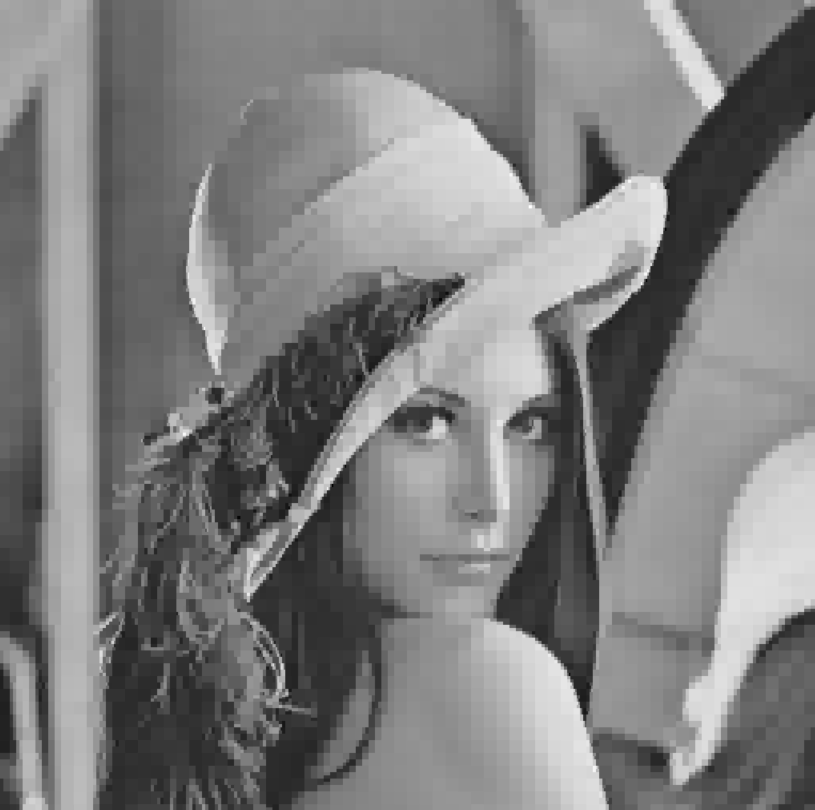
\includegraphics[width=\linewidth]{Lena_70.png}
			
			\vspace{0.2cm}
			{\color{bleu}\bfseries $\lambda = 70$}
			
			\column{0.33\textwidth}
			\centering
			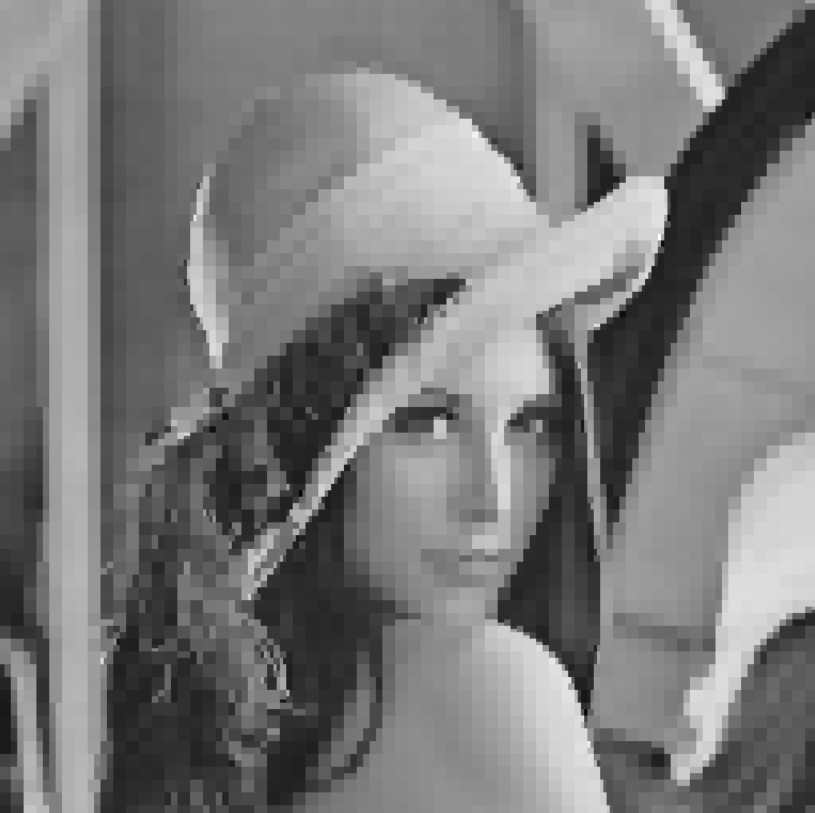
\includegraphics[width=\linewidth]{Lena_150.png}
			
			\vspace{0.2cm}
			{\color{bleu}\bfseries $\lambda = 150$}
			
		\end{columns}
		
		\vspace{0.5cm}
		
		\begin{center}
			\small
			Plus $\lambda$ est élevé, plus  un grand nombre de coefficients sont supprimés.
		\end{center}
		
	\end{frame}
	
	
	\begin{frame}{III -- Résultats expérimentaux : Comparaison des seuils}
		
		\centering
		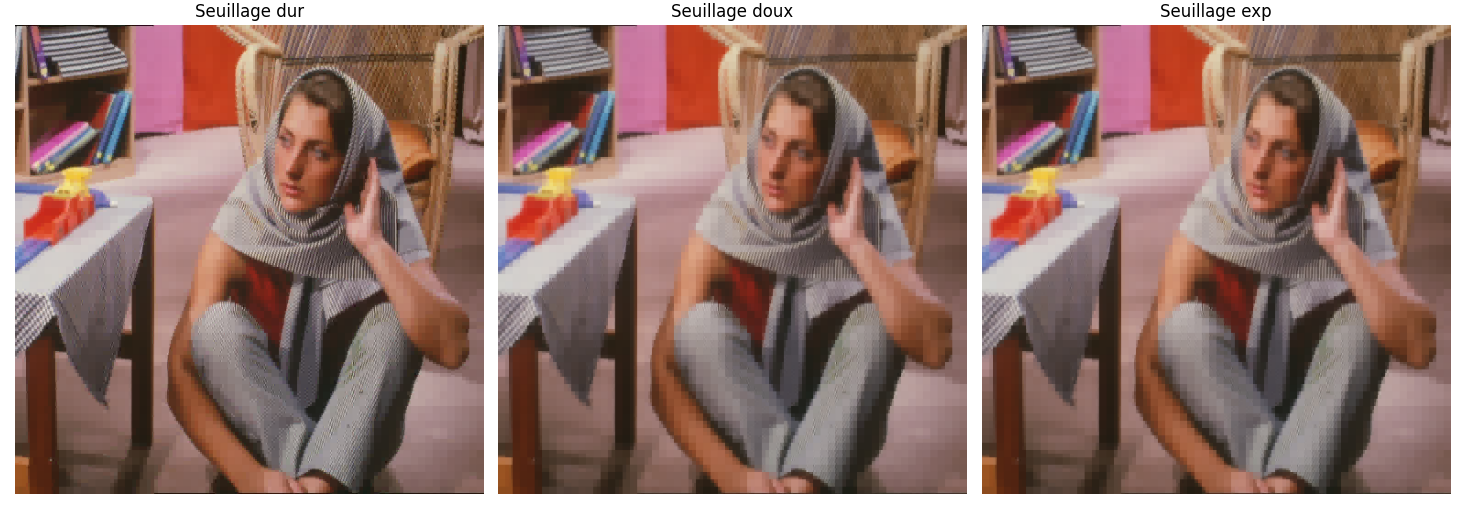
\includegraphics[scale=1.4, width=\linewidth]{barbara_cool.png}
		
		\begin{alertblock}{Analyse des résultats}
			\begin{enumerate}
				\item Le seuillage $\texttt{dur}$ laisse transparaître les discontinuités dans l'image.
				\item Le seuillage $\texttt{doux}$ tend à lisser l'image et à l'obscurcir légèrement.
				\item Le seuillage $\texttt{exp}$ est expérimental et prolonge par continuité les branches entre le seuillage $\texttt{dur}$ et $\texttt{doux}$ de façon à \emph{garder le meilleur de chaque}.
				\item Chaque seuillage peut être intéressant pour des images différentes. 
			\end{enumerate}
		\end{alertblock}
		
	\end{frame}
	
	\subsubsection{Résultats expérimentaux}
	
	\begin{frame}[t]{III — Résultats expérimentaux : taux de compression}
		
		\vspace{-0.2cm}
		
		\textbf{Configuration :} image $512\times512$, Haar, $L=4$ niveaux, seuillage dur.
		
		\vspace{-0.3cm}
		
		\[ \mathrm{PSNR}=10\log_{10}\!\dfrac{255^2}{\mathrm{MSE}}  = \text{Indicateur de différence par rapport à l'image originale.} \]
		\medskip
		\centering
		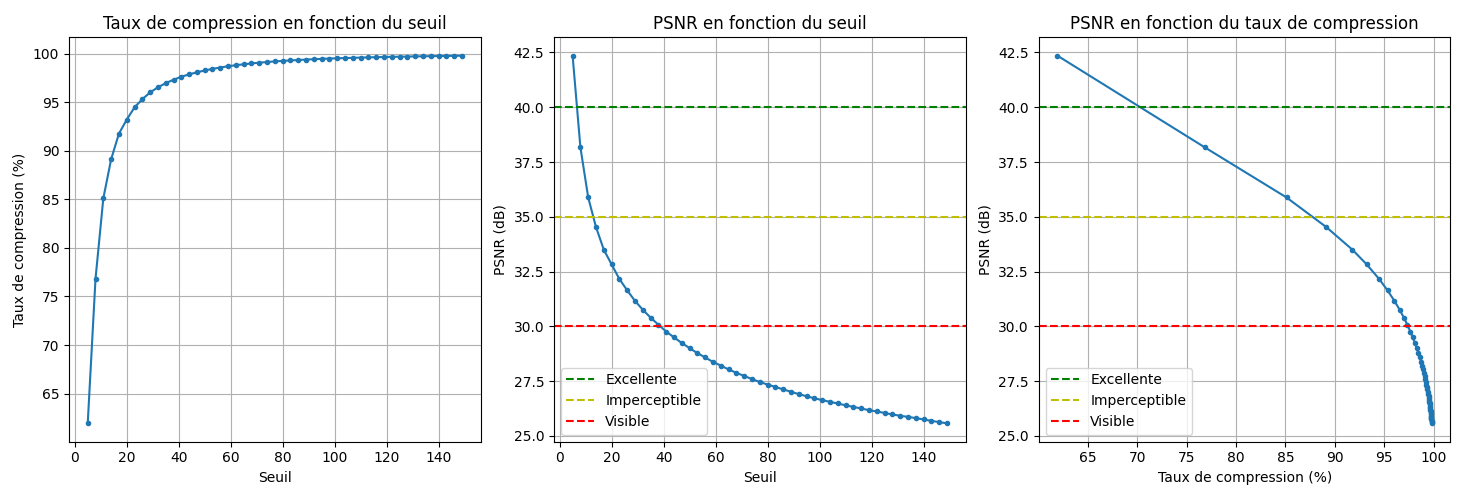
\includegraphics[width=\linewidth]{PSNR.png}
		
		\begin{alertblock}{Conclusion sur les effets du seuillage}
			\begin{enumerate}
				\item La qualité de l'image est une fonction décroissante du seuil.
				\item On peut expérimentalement déterminer un seuil optimal pour une dite configuration.
			\end{enumerate} 
		\end{alertblock}
		
	\end{frame}
	
	\begin{frame}[t]{III - Résultats expérimentaux : Distribution des coeffs}
		
		\begin{columns}[T]
			\column{0.5\textwidth}
			\centering
			\textbf{Ondelette de Haar}
			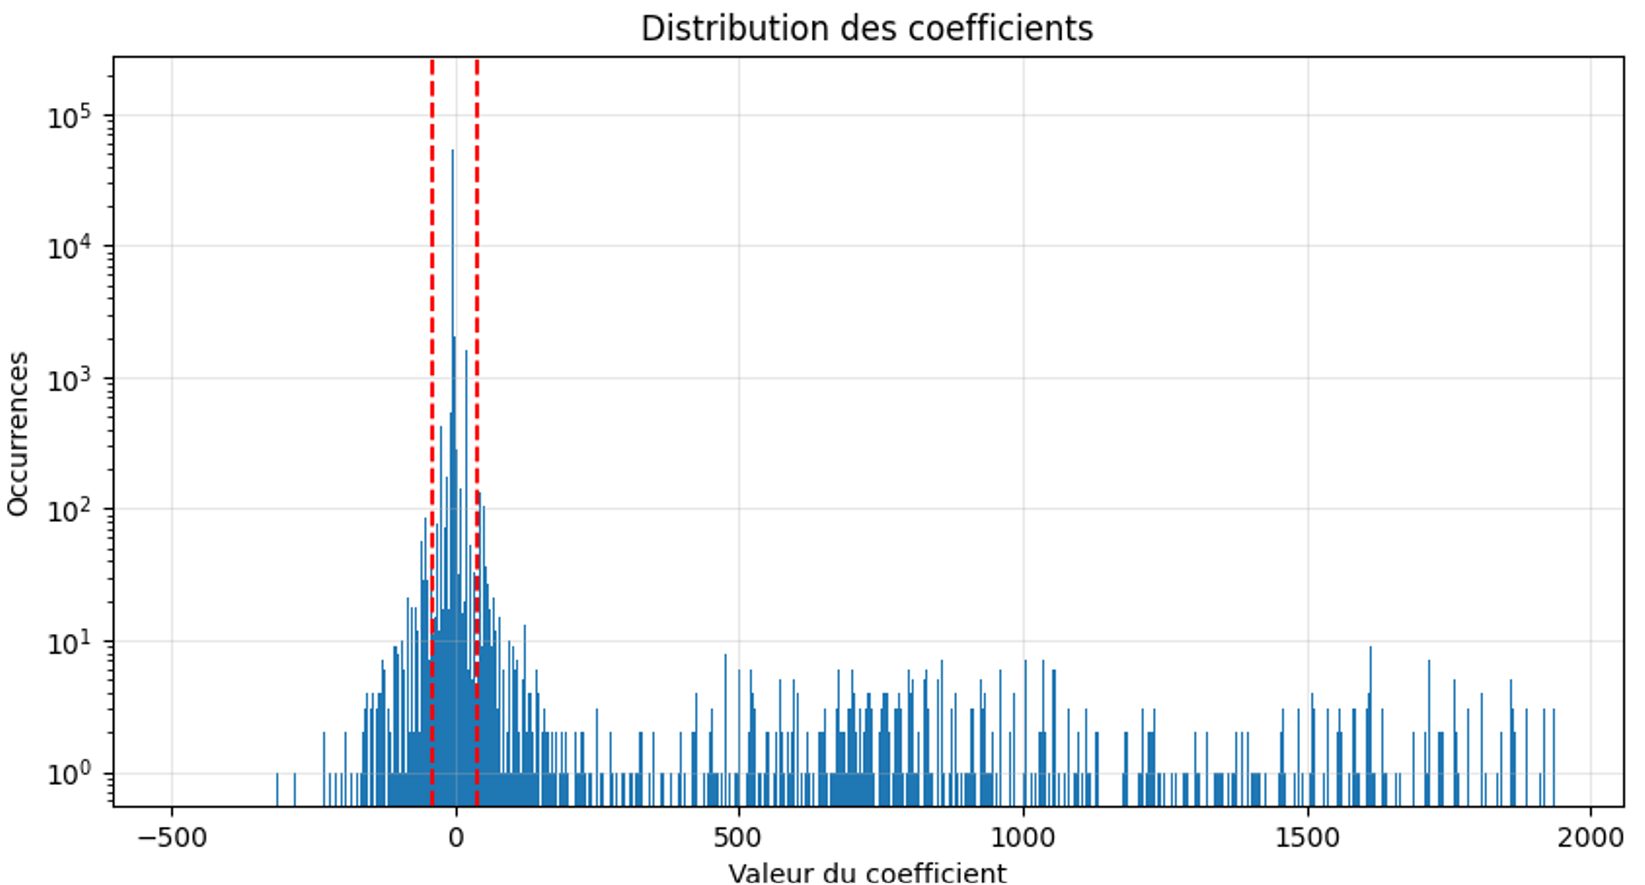
\includegraphics[width=\linewidth]{distri_coeffs_haar}
			
			\column{0.5\textwidth}
			\centering
			\textbf{Ondelette de Daubechies}
			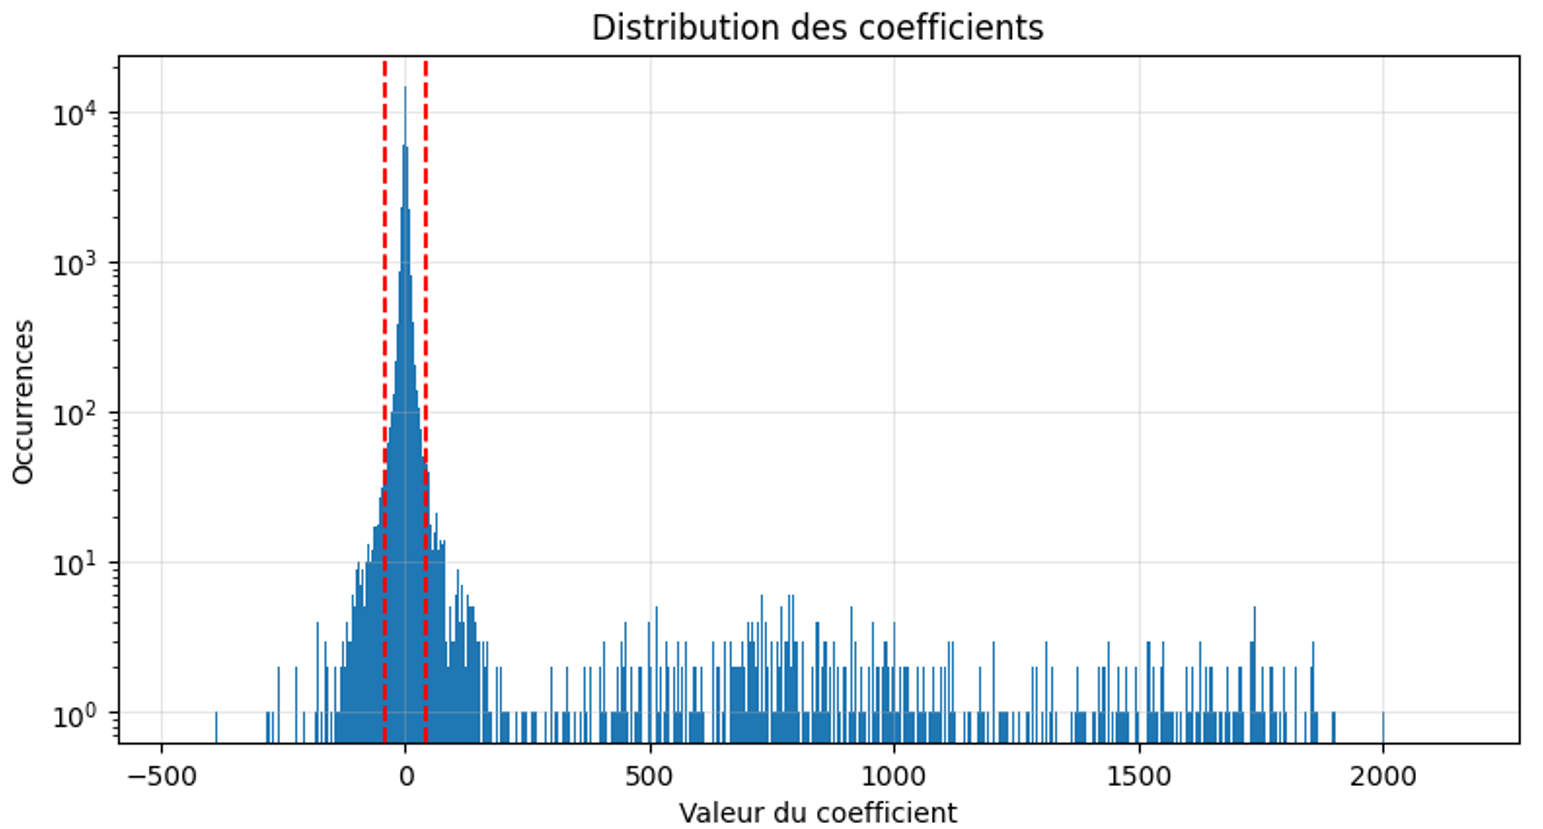
\includegraphics[width=\linewidth]{distri_coeffs_daubechies}
		\end{columns}
		
		\vspace{0.cm}
		
		\begin{columns}[C]
			\column{0.48\textwidth}
			\centering
			
\includegraphics[width=0.8\linewidth]{pernette}
			
			\column{0.52\textwidth}
			\raggedleft
			
			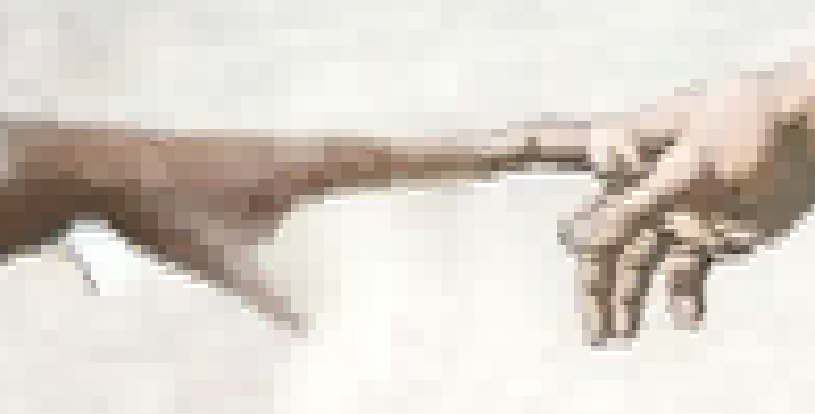
\includegraphics[scale=0.305]{main_haar} \quad (Avec Haar) \qquad
			
			
			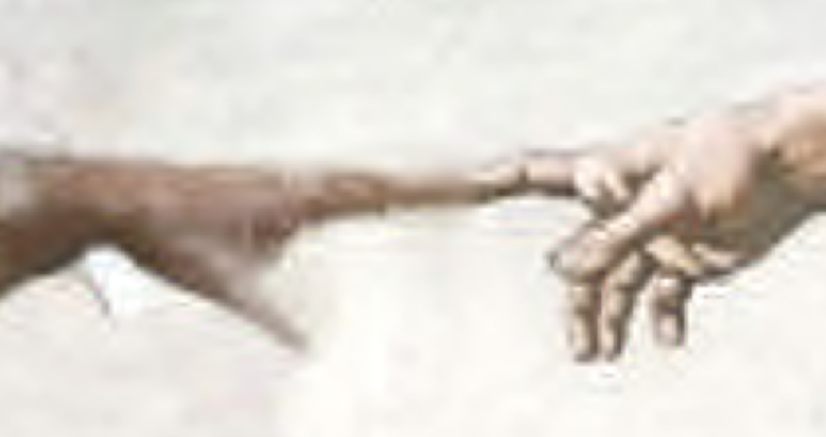
\includegraphics[scale=0.2985]{main_daubechies} \quad (Daubechies)
		\end{columns}
		
	\end{frame}
	
	\begin{frame}[t]{III - Résultats expérimentaux : Comparaison ondelettes} 
		\centering 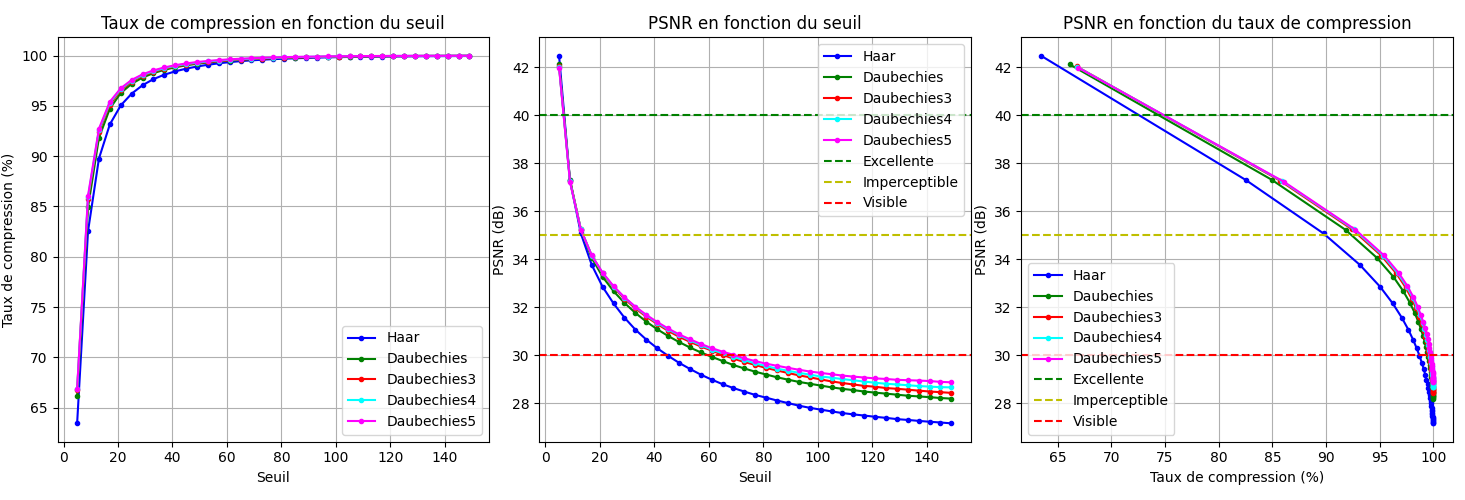
\includegraphics[scale=1.4, width=\linewidth]{compa_ondelettes.png} 
		\medskip 
		
		\begin{alertblock}{Analyse des résultats} 
			\begin{enumerate} 
				\item Le choix de l'ondelette importe ; pour JPEG : CDF 9/7. 
				\item Certaines ondelettes permettent de comprimer plus sans perdre davantage de détails.
			\end{enumerate} 
		\end{alertblock} 
	\end{frame}
	
	
	\subsection{Complexité algorithmique}
	\begin{frame}{III — Complexité de la transformée de Haar}
		
		\textbf{L'algorithme pyramidal}\\[2pt]
		À chaque niveau $j$, on traite un signal deux fois plus court que le précédent.
		
		\begin{columns}[T]
			\column{0.52\textwidth}
			\begin{block}{Calcul de la complexité 1D}
				Pour un signal de taille $N$ :
				\begin{itemize}
					\item Étape 1 : $N$ opérations (sommes/diff)
					\item Étape 2 : $N/2$ opérations
					\item Étape $k$ : $N/2^{k-1}$ opérations
				\end{itemize}
				Total : \[\sum_{k=0}^{\lfloor 
					\log_2 N \rfloor 
				} \frac{N}{2^k} = N (1 + \frac{1}{2} + \frac{1}{4} + \dots) < \mathbf{2N}\]
			\end{block}
			
			\begin{itemize}
				\item \textbf{Complexité 1D :} $O(N)$
				\item \textbf{Complexité 2D :} $O(N^2)$ \\ (\emph{linéaire} en nombre de pixels)
			\end{itemize}
			
			\column{0.44\textwidth}
			\centering
			\textbf{Comparaison avec Fourier}\\[4pt]
			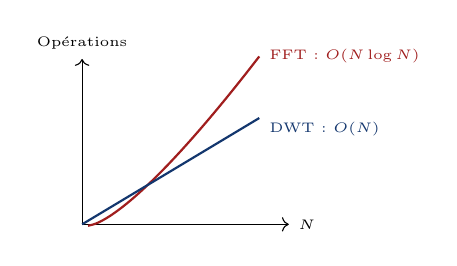
\begin{tikzpicture}[scale=0.75, font=\tiny]
				\draw[->] (0,0) -- (3.5,0) node[right]{$N$};
				\draw[->] (0,0) -- (0,2.8) node[above]{Opérations};
				
				% Courbe FFT N log N
				\draw[domain=0.1:3.0, smooth, variable=\x, rouge, thick] plot ({\x}, {0.35*\x*ln(5*\x)}) node[right]{FFT : $O(N \log N)$};
				
				% Courbe Ondelette N
				\draw[domain=0:3.0, smooth, variable=\x, bleu, thick] plot ({\x}, {0.6*\x}) node[right, yshift=-4pt]{DWT : $O(N)$};
			\end{tikzpicture}
			\begin{alertblock}{Atout majeur}
				Contrairement à la FFT, la transformée de Haar n'utilise \textbf{aucune multiplication complexe}, seulement des additions et des soustractions.
			\end{alertblock}
		\end{columns}
		
	\end{frame}
	
	%%═══════════════════════════════════════════════════════════════════════
	%%═══════════════════════════════════════════════════════════════════════
	\section{IV. Conclusion}
	%%═══════════════════════════════════════════════════════════════════════
	
	%%═══════════════════════════════════════════════════════════════════════
	%% DIAPO 18 — Bilan
	%%═══════════════════════════════════════════════════════════════════════
	\section*{Conclusion}
	
	\begin{frame}{Conclusion et perspectives}
		\vspace{-0.1em}
		
		%% ─── BILAN DU TRAVAIL ─────────────────────────────────────────────
		{\large\bfseries\color{bleu} Bilan du TIPE}
		\nopagebreak
		\vspace{0.2em}
		{\color{bleumed}\hrule height 1pt}
		\vspace{0.6em}
		
		\begin{itemize}
			\item[\color{bleu}\blacktriangleright] \textbf{Représentation creuse idéale :} La double localisation (spatiale et fréquentielle) des ondelettes permet de capturer efficacement à la fois les zones lisses et les contours nets des images.
			\item[\color{bleu}\blacktriangleright] \textbf{Algorithme linéaire :} Grâce à l'analyse multi-résolution (AMR), les décompositions et reconstructions s'effectuent en temps $\mathcal{O}(N)$.
			\item[\color{bleu}\blacktriangleright] \textbf{Supériorité technique :} La DWT préserve parfaitement l'énergie ; et compresse les images très efficacement.
		\end{itemize}
		
		\vspace{1.0em}
		
		%% ─── PERSPECTIVES ─────────────────────────────────────────────────
		{\large\bfseries\color{bleu} Perspectives d'ouverture}
		\nopagebreak
		\vspace{0.2em}
		{\color{bleumed}\hrule height 1pt}
		\vspace{0.6em}
		
		\begin{itemize}
			\item[\color{rouge}\blacktriangleright]
			\textbf{Débruiter un signal :} Seuiller sur les coefficients d'ondelettes un signal à bruit gaussien et le reconstruire. (Donoho–Johnstone)
			\item[\color{rouge}\blacktriangleright] \textbf{Hybridation avec le Deep Learning :} Coupler les banques de filtres en ondelettes avec des réseaux de neurones convolutifs (CNN) modernes pour le débruitage et la super-resolution d'images.
			\item[\color{rouge}\blacktriangleright] \textbf{Extension 3D et vidéo :} Généraliser au traitement de volumes tridimensionnels (imagerie médicale IRM) ou à la compression temporelle de flux vidéo.
		\end{itemize}
	\end{frame}
	
	%%═══════════════════════════════════════════════════════════════════════
	\appendix
	%%═══════════════════════════════════════════════════════════════════════
	
	%%═══════════════════════════════════════════════════════════════════════
	%% ANNEXE B — Implémentation Python
	%%═══════════════════════════════════════════════════════════════════════
	\begin{frame}[fragile]{Annexe — Implémentation : Noyau 1D et 2D (Haar)}
		\begin{columns}[T]
			%% --- COLONNE GAUCHE : DIRECTE ---
			\column{0.48\textwidth}
			{\footnotesize\bfseries\color{bleu} �� Analyse Directe (Lignes/Colonnes)}
			\vspace{0.3em}
			\begin{lstlisting}[basicstyle=\tiny\ttfamily,frame=single,language=Python,numbers=none]
				def transformation_1d(self, x):
				n = len(x) // 2
				approx = (x[0::2] + x[1::2]) / np.sqrt(2)
				detail = (x[0::2] - x[1::2]) / np.sqrt(2)
				return np.concatenate([approx, detail])
				
				def transformation_2d(self, mat):
				res = np.zeros_like(mat, dtype=float)
				# 1) Transformation des lignes
				for i in range(mat.shape[0]):
				res[i, :] = self.transformation_1d(mat[i, :])
				# 2) Transformation des colonnes
				for j in range(mat.shape[1]):
				res[:, j] = self.transformation_1d(res[:, j])
				return res
			\end{lstlisting}
			
			%% --- COLONNE DROITE : INVERSE ---
			\column{0.48\textwidth}
			{\footnotesize\bfseries\color{rouge} �� Synthèse Inverse (Recomposition)}
			\vspace{0.3em}
			\begin{lstlisting}[basicstyle=\tiny\ttfamily,frame=single,language=Python,numbers=none]
				def transformation_1d_inverse(self, c):
				n = len(c) // 2
				approx, detail = c[:n], c[n:]
				x = np.empty(len(c))
				x[0::2] = (approx + detail) / np.sqrt(2)
				x[1::2] = (approx - detail) / np.sqrt(2)
				return x
				
				def transformation_2d_inverse(self, mat):
				res = np.zeros_like(mat, dtype=float)
				# 1) Inverse sur les colonnes
				for j in range(mat.shape[1]):
				res[:, j] = self.transformation_1d_inverse(mat[:, j])
				# 2) Inverse sur les lignes
				for i in range(mat.shape[0]):
				res[i, :] = self.transformation_1d_inverse(res[i, :])
				return res
			\end{lstlisting}
		\end{columns}
	\end{frame}
	
	%%═══════════════════════════════════════════════════════════════════════
	%% CODES PYTHON — SLIDE 2 : CASCADE MULTI-RESOLUTION (FORWARD / INVERSE)
	%%═══════════════════════════════════════════════════════════════════════
	\begin{frame}[fragile]{Annexe — Analyse Multi-Résolution (AMR)}
		\begin{columns}[T]
			%% --- COLONNE GAUCHE : FORWARD ---
			\column{0.48\textwidth}
			{\footnotesize\bfseries\color{bleu} �� Décomposition en Cascade (\texttt{forward})}
			\vspace{0.3em}
			\begin{lstlisting}[basicstyle=\tiny\ttfamily,frame=single,language=Python,numbers=none]
				def forward(self):
				res = self.img.copy()
				n, p = res.shape
				for _ in range(self.levels):
				# Applique la T2D sur le sous-bloc
				res[:n, :p] = self.transformation_2d(res[:n, :p])
				# On restreint au quadrant bas-frequence
				n //= 2
				p //= 2
				return res
			\end{lstlisting}
			
			%% --- COLONNE DROITE : INVERSE ---
			\column{0.48\textwidth}
			{\footnotesize\bfseries\color{rouge} �� Reconstruction (\texttt{inverse})}
			\vspace{0.3em}
			\begin{lstlisting}[basicstyle=\tiny\ttfamily,frame=single,language=Python,numbers=none]
				def inverse(self, coeffs):
				res = coeffs.copy()
				# Taille du plus petit quadrant initial
				n = len(res) // 2**(self.levels - 1)
				p = len(res[0]) // 2**(self.levels - 1)
				
				for _ in range(self.levels):
				# Remonte d'un niveau d'echelle
				res[:n, :p] = self.transformation_2d_inverse(res[:n, :p])
				n *= 2
				p *= 2
				return res
			\end{lstlisting}
		\end{columns}
	\end{frame}
	
	%%═══════════════════════════════════════════════════════════════════════
	%% ANNEXE A — DCT (ancienne diapo 5)
	%%═══════════════════════════════════════════════════════════════════════
	\begin{frame}{Annexe — JPEG : la DCT par blocs}
		
		\textbf{Idée} : se placer dans une base \emph{fréquentielle} adaptée,
		puis garder seulement les coefficients importants.
		
		\medskip
		\begin{columns}[T]
			\column{0.60\textwidth}
			\textbf{Principe de JPEG}
			\begin{enumerate}
				\item Découper l'image en blocs $8\times 8$
				\item Projection des coeffs sur une base de cosinus (adapdée aux fréquences) :
				\[\textstyle
				C_{p,q} = \lambda_p\lambda_q
				\sum_{n,m} F[n,m]\cos\!\frac{\pi p(n+\tfrac{1}{2})}{8}
				\cos\!\frac{\pi q(m+\tfrac{1}{2})}{8}
				\]
				\item Seuillage des HF (invisible à l'oeil nu)
				\item Coder les coefficients restants (Huffman)
			\end{enumerate}
			
			\column{0.36\textwidth}
			\vspace*{-0.8cm}
			\hfill
			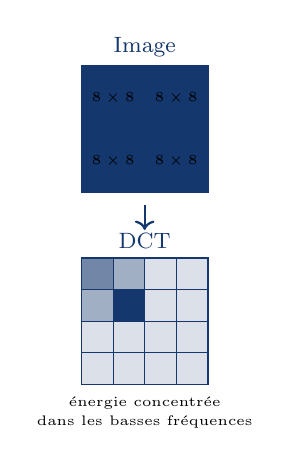
\begin{tikzpicture}[scale=0.8,font=\scriptsize,yshift=0.5cm]
				
				\draw[fill=bleulight,bleu,thick] (0,0) rectangle (2,2);
				\draw[bleu] (1,0)--(1,2);
				\draw[bleu] (0,1)--(2,1);
				
				\foreach \x/\y in {0.5/1.5,1.5/1.5,0.5/0.5,1.5/0.5}
				\node[font=\tiny] at (\x,\y) {$8\times8$};
				
				\node[above,font=\footnotesize,bleu] at (1,2)
				{Image};
				
				\draw[->,bleu,thick] (1,-0.2)--(1,-0.6);
				
				\begin{scope}[yshift=-3.05cm]
					
					\draw[fill=bleulight!70,bleu,thick]
					(0,0) rectangle (2,2);
					
					\fill[bleu!60] (0,1.5) rectangle (0.5,2);
					\fill[bleu!40] (0,1.0) rectangle (0.5,1.5);
					\fill[bleu!40] (0.5,1.5) rectangle (1.0,2);
					
					\fill[bleu!15] (0,0) rectangle (2,1.0);
					\fill[bleu!15] (1.0,1.0) rectangle (2,2);
					
					\draw[bleu,thin] (0,0) grid[step=0.5] (2,2);
					
					\node[above,font=\footnotesize,bleu]
					at (1,2) {DCT};
					
					\node[font=\tiny,below]
					at (1,-0.05)
					{énergie concentrée};
					
					\node[font=\tiny,below]
					at (1,-0.35)
					{dans les basses fréquences};
					
				\end{scope}
				
			\end{tikzpicture}
		\end{columns}
		
		\begin{alertblock}{Défaut de JPEG à fort taux de compression}
			Ce traitement crée des
			\textbf{artefacts de blocs} : les discontinuités aux frontières
			deviennent visibles.\\[3pt]
			\emph{Cause :} la DCT ne prend pas en compte la continuité entre blocs.
		\end{alertblock}
		
	\end{frame}
	
	%%═══════════════════════════════════════════════════════════════════════
	%% SECTION — SOURCES & RÉFÉRENCES
	%%═══════════════════════════════════════════════════════════════════════
	\section*{Sources}
	
	\begin{frame}{Sources et Références}
		\vspace{-0.6em}
		
		%% ─── COURS & ARTICLES SCIENTIFIQUES ────────────────────────────────
		{\large\bfseries\color{bleu} Cours et Articles Scientifiques}
		\nopagebreak
		\vspace{0.1em}
		{\color{bleumed}\hrule height 1pt}
		\vspace{0.4em}
		
		\begin{itemize}
			\item[\color{bleu}\blacktriangleright] \textbf{Pr. Valérie Perrier :} \emph{Cours sur la Transformée par Ondelettes (Vols. 1 à 5)}. Une référence universitaire complète pour (AMR).\\
			\footnotesize\texttt{https://membres-ljk.imag.fr/Valerie.Perrier/PUBLI/Cours1-VP.pdf} 
			
			\item[\color{bleu}\blacktriangleright] \textbf{M. Cagnazzo (IMT) :} \emph{Wavelet Denoising}. \\ Analyse approfondie des techniques de débruitage d'images par seuillage d'ondelettes.\\
			\footnotesize\texttt{https://cagnazzo.wp.imt.fr/files/2018/04/wavelet\_denoising.pdf}
			
			\item[\color{bleu}\blacktriangleright] \textbf{M. Duffaud (CPGE Paradise) :} \emph{Compression d'images par ondelettes}. \\ Support d'étude de cas et d'implémentation en TIPE.\\
			\footnotesize\texttt{https://cpge-paradise.com/TIPE/martin\_duffaud/PPT\_duffaud.pdf}
		\end{itemize}
		
		\vspace{0.8em}
		
		%% ─── VULGARISATION & CONTENUS NUMÉRIQUES ───────────────────────────
		{\large\bfseries\color{bleu} Vulgarisation et Ressources Numériques}
		\nopagebreak
		\vspace{0.1em}
		{\color{bleumed}\hrule height 1pt}
		\vspace{0.4em}
		
		\begin{itemize}
			\item[\color{rouge}\blacktriangleright] \textbf{El Jj (YouTube) :} \emph{Une ondelette pour les compresser toutes}. \\Présentation intuitive et visuelle des ondelettes de Haar et Daubechies.\\
			\footnotesize\texttt{https://www.youtube.com/watch?v=vpmlGMZSpvQ}
			
			\item[\color{rouge}\blacktriangleright] \textbf{Wikipédia :} \emph{Standard de compression et d'analyse JPEG 2000}.\\ Principes théoriques de la quantification et de l'encodage entropique adaptatif.\\
			\footnotesize\texttt{https://fr.wikipedia.org/wiki/JPEG\_2000}
		\end{itemize}
	\end{frame}
	
\end{document}